\chapter{Version Control}

\section{Software Versions}

No writer can finish a good book in one shot. A book needs to be
writen section by section and chapter by chapter. The writing is
likely reviewed and revised multiple times. If you watch a movie DVD,
you can find {\it Deleted Scenes}--- the sections that have been made
but never used in the actual movie.  Any non-trivial work needs to be
created gradually and improved over and over again before it is ready.
Developing software is no different: functionality is added
gradually. Sometimes, finished functions need to change because
customers' needs have changed, competitors have introduced new
features and modifications are needed, new regulations are announced,
or new standards are issued. All of these mean that software must be
developed in small pieces; these pieces are called {\it version}.

There is no widely accepted definition of a version, just like there
is no specific definition what should be considered as a chapter in a
book. One may consider each additional line as a new version while
another may consider a completely implemented and fully tested feature
as a version. Generally speaking, a version should be self-contained
and complete unit, like a section or a chapter in a book.  The tools
that manage versions are called {\it version control}.  When multiple
work together, version control becomes essential to ensure proper
coordination.

There are many version control systems, such {\tt CVS} (concurrent
version system) and {\tt SVN} (subversion).  This book uses {\tt git}
for version control. It is a {\it distributed} version control system,
meaning that there can be two types of {\it repositories}: One is on
each user's computer; the other is shared by all users. The advantage
of a distributed version control system will become clear after
explaining how people collaborate developing software.

The version control system {\tt git} is a set of programs managing
files.  You can run {\tt git} on your own computer. You can also set
up a {\tt git} server shared by multiple people. Alternatively, you
can use websites that offer version control functions; examples
include {\tt github.com} and {\tt bitbucket.org}.  This book uses {\tt
  github} as an example.  You can find entire books talking about {\tt
  git} as well as thousands of web postings about how to use {\tt
  github}. {\tt git} has many different functions and {\tt github}
offers many different ways to accomplish the same goals.  This book
does not intend to replace those materials.  Instead, this book
provides enough details for common needs.  Readers interested knowing
more can easily find additional documentations.

\section{\tt github}

This book chooses {\tt github} for three reasons: (1) It is widely used.
(2) It is free for education purposes. (3) It is supported by many  tools
other than the {\tt github} website.

\begin{figure}[h] \centering
 \subfigure[]
{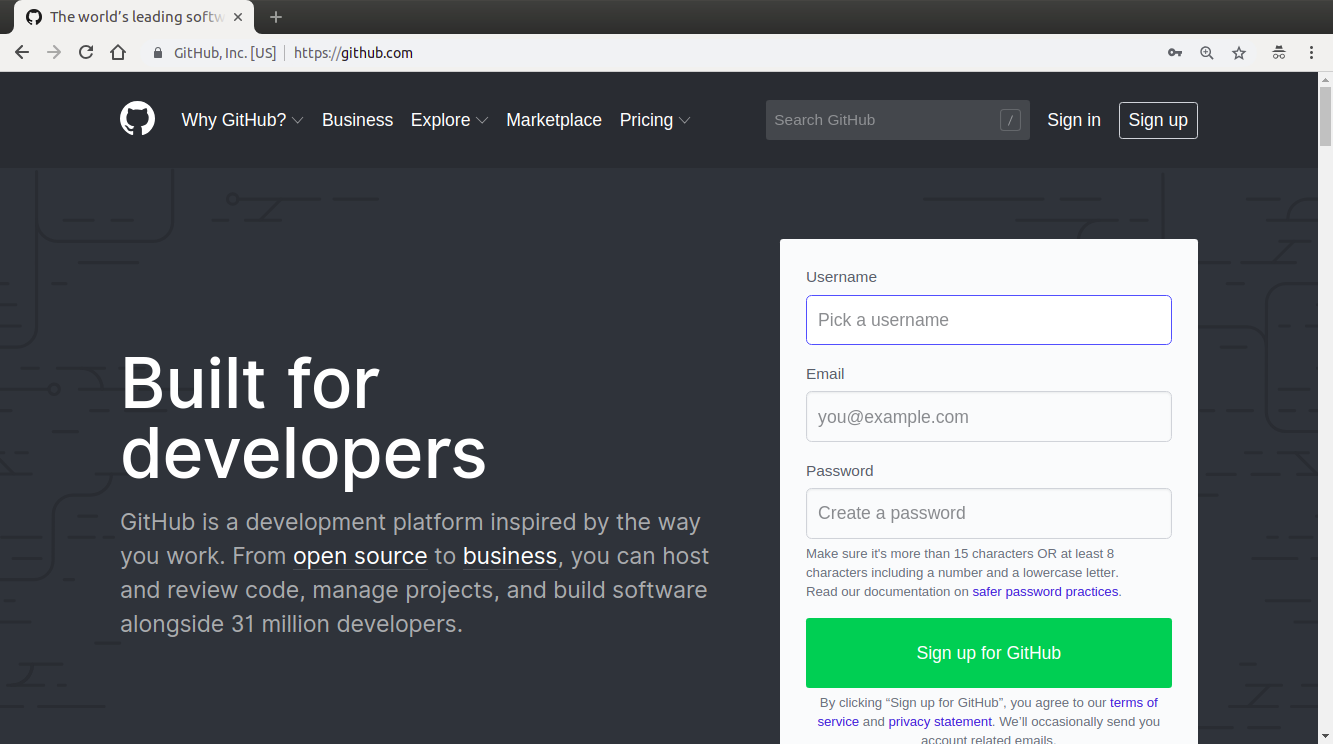
\includegraphics[width=4in]{\thischapterpath/figures/github1.png}}
  \subfigure[]
{
\includegraphics[width=4in]{\thischapterpath/figures/github2.png}}
\caption{(a) {\tt github} website. (b) Students and teachers can apply for free repositories.}
\label{fig:github}
\end{figure}
